\documentclass[10pt,pdf,hyperref={unicode}]{beamer}
\usepackage{amsmath, amsfonts}
\usepackage[utf8]{inputenc}
\usepackage[russian]{babel}
\usepackage{graphicx}
\usepackage{animate}
%\usetheme{Madrid}

\begin{document}
\begin{frame}
\begin{center}
    Московский государственный университет имени М. В. Ломоносова
    \bigskip
    Факультет Вычислительной Математики и Кибернетики\\[5mm]

    \textsf{\large\bfseries
        Решение задачи диффузии-конвекции в жидкости с пульсирующим источником
    }\\[5mm]

    \begin{flushright}
        \parbox{0.5\textwidth}{
            Выполнил:\\
            студент 4 курса 427 группы\\
            \emph{Е. Ю. Пышнограев}\\[3mm]
            Научный руководитель:\\
            д.ф-м.н., профессор\\
            \emph{М. М. Хапаев}
        }
    \end{flushright}

    \vspace{\fill}
    Москва, 2013
\end{center}
\end{frame}

\begin{frame}
  \frametitle{Введение}
  \begin{itemize}
    \item Процесс диффузии вещества в жидкости
      \pause
    \item Детальность описания задачи, переход от простого к сложному
  \end{itemize}
\end{frame}

\begin{frame}
  \frametitle{Введение}
  \begin{itemize}
    \item Простейшая модель
      \begin{equation*}
        u_t = a^2 u_{xx}
      \end{equation*}
      \begin{figure}[ht]
        \begin{center}
          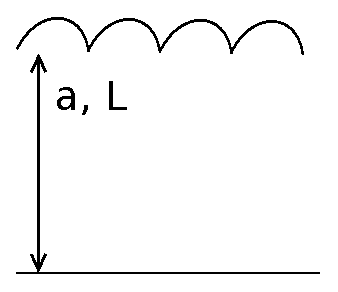
\includegraphics[width=5cm]{int1.eps}
        \end{center}
      \end{figure}
  \end{itemize}
  \pause
  Что можно добавить в модель чтобы сделать ее достовернее?
\end{frame}

\begin{frame}
  \frametitle{Введение}
  Что можно добавить в модель чтобы сделать ее достовернее?
  \begin{columns}
    \column{0.5 \textwidth}
    \begin{itemize}
      \item Добавим конвективное слагаемое
    \end{itemize}
    \begin{equation*}
      u_t = a^2 u_{xx} + w u_x
    \end{equation*}
      \begin{figure}[ht]
        \begin{center}
          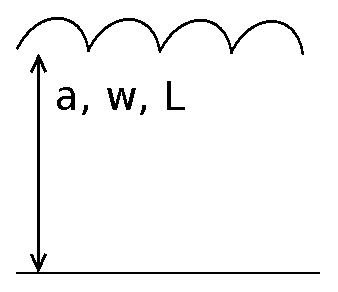
\includegraphics[width=3cm]{int2.eps}
        \end{center}
      \end{figure}

    \pause
    \column{0.5 \textwidth}
    \begin{itemize}
      \item Сделаем область многослойной
    \end{itemize}
    \begin{equation*}
      u_t = a(x) u_{xx}
    \end{equation*}
      \begin{figure}[ht]
        \begin{center}
          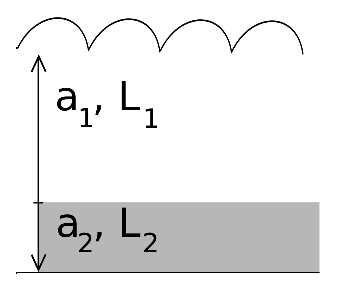
\includegraphics[width=3cm]{int3.eps}
        \end{center}
      \end{figure}
  \end{columns}
\end{frame}

\begin{frame}
  \frametitle{Постановка задачи}

  \begin{columns}
    \column{0.4 \textwidth}
  \begin{equation*}
   u_t = wu_x + a^2 u_{xx},
  \end{equation*}
  \begin{equation*}
   u(x,0) = 0,
  \end{equation*}
  \begin{equation*}
    \left\{
    \begin{aligned}
      & u(-l_1,t) = 1 - \cos \omega t, \\
      & u_x(l_2,t) = 0, \\
      & u(-0, t) = u(+0, t), \\
      & a_1^2 u_{x}(-0, t) = a_2^2 u_{x}(+0, t). \\
    \end{aligned}
    \right.
  \end{equation*}
    \column{0.6 \textwidth}
  \begin{figure}[ht]
    \begin{center}
      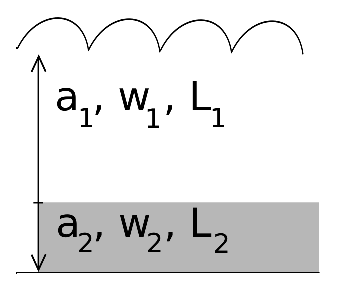
\includegraphics[width=5cm]{int4.eps}
    \end{center}
  \end{figure}
  \end{columns}
\end{frame}

\begin{frame}
  \frametitle{Возможные подходы}
  \begin{columns}
    \column{0.5 \textwidth}
    Численный метод
    \begin{itemize}
      \item Применим в большинстве случаев, обычно не требует сложных предварительных выкладок
      \item Неизвестен общий вид искомой функции
      \item Часто необходимо много вычислительных ресурсов
    \end{itemize}

    \column{0.5 \textwidth}
    Аналитический метод
    \begin{itemize}
      \item Может быть использован не всегда, при решении часто бывают трудности
      \item Если все получилось, то получаем явную формулу для результата
      \item Точное решение может использоваться для проверки адекватности численного метода для задачи
    \end{itemize}
  \end{columns}
\end{frame}

\begin{frame}
  \frametitle{Этапы решения}
  Решение задачи будем находить методом конечных интегральных преобразований:
  \begin{itemize}
    \item Переход к однородным граничным условиям
    \item Разделение переменных
    \item Составление задачи Штурма--Лиувилля
    \item Вывод уравнения для собственных чисел
    \item Нахождение общего вида собственных функций
    \item Вычисление веса, с которым ортогональны собственные функции
    \item Проведение интегрального преобразования
    \item Нахождение временной составляющей решения
    \item Получение окончательного ответа
  \end{itemize}
\end{frame}

\begin{frame}
  \frametitle{Переход к однородным граничным условиям} 
  Производим замену
  \begin{equation*}
    u(x,t) = U(x,t) + (1 - \cos \omega t).
  \end{equation*}
  В результате приходим к новому уравнению, начальному и граничным условиям
  \begin{equation*}
    U_t(x,t) = w U_x(x,t) + a^2 U_{xx}(x,t) - \omega\sin\omega t,
  \end{equation*}
  \begin{equation*}
    U(x,0) = 0,
  \end{equation*}
  \begin{equation*}
    \left\{
    \begin{aligned}
      & U(-l_1,t) = 0, \\
      & U_x(l_2,t) = 0, \\
      & U(-0, t) = U(+0, t), \\
      & a_1^2 U_{x}(-0, t) = a_2^2 U_{x}(+0, t). \\
    \end{aligned}
    \right.
  \end{equation*}
\end{frame}

\begin{frame}
  \frametitle{Разделение переменных}
  Пусть $ U(x,t)=\theta(t)\varphi(x) $, тогда
  \begin{equation*}
    \frac{\theta'}{\theta}=\frac{a^2\varphi''+w\varphi'}{\varphi}=s.
    \label{eq:1}
  \end{equation*}
  Константа $ s $ не может быть положительной, в противном случае функция $\theta(t)$ будет не ограничена, что противоречит физическому смыслу задачи. Ввиду этого, можно принять
  \begin{equation*}
    s=-\lambda^2.
    \label{eq:2}
  \end{equation*}
\end{frame}

\begin{frame}
  \frametitle{Составление задачи Штурма--Лиувилля}
  В результате разделения переменных получаем задачу Штурма--Лиувилля для $\varphi(x)$:
  \begin{equation*}
    a^2 \varphi''(x) + w \varphi'(x) + \lambda^2\varphi(x)=0 
  \end{equation*}
  с внешними граничными условиями и условиями сопряжения:
  \begin{equation*}
    \left\{
    \begin{aligned}
      & \varphi_1(-l_1) = 0, \\
      & \varphi_2'(l_2) = 0, \\
      & \varphi_1(0) = \varphi_2(0), \\
      & a_1^2 \varphi_1'(0) = a_2^2 \varphi_2'(0). \\
    \end{aligned}
    \right.
  \end{equation*}
\end{frame}

\begin{frame}
  \frametitle{Составление задачи Штурма--Лиувилля}
  Для того чтобы исключить из уравнения слагаемое $w\varphi'(x)$, производим замену 
  \begin{equation*}
    \varphi(x) = \psi(x) e^{- \mu x},\ \text{где}\ \mu=\mu(x) = \left\{
      \begin{aligned}
        & \mu_1 = \frac{w_1}{2a_1^2}\ \text{при}\ x \in [-l_1;0), \\
        & \mu_2 = \frac{w_2}{2a_2^2}\ \text{при}\ x \in [0;l_2]. \\
      \end{aligned}
      \right.
  \end{equation*}
  В итоге получаем новое уравнение
  \begin{equation*}
    a^2\psi''(x) + (\lambda^2 - \mu^2a^2) \psi(x) = 0
    \label{eq:3}
  \end{equation*}
  и новые граничные условия
  \begin{equation*}
    \left\{
    \begin{aligned}
      & \psi_1(-l_1) = 0, \\
      & \psi_2'(l_2) - \mu\psi_2(l_2) = 0, \\
      & \psi_1(0) = \psi_2(0), \\
      & a_1^2(\psi_1'(0) - \mu\psi_1(0)) =  a_2^2(\psi_2'(0) - \mu\psi_2(0)). \\
    \end{aligned}
    \right.
    \label{}
  \end{equation*}
\end{frame}

\begin{frame}
  \frametitle{Уравнение для собственных чисел}
  Пусть, для определенности, $\mu_1 a_1 < \mu_2 a_2$.
  Вариант $\mu_1 a_1 < \mu_2 a_2$ --- частный случай рассмотренного ниже.
  Уравнение имеет разный вид на трех промежутках:
  \begin{enumerate}
    \item $ 0 \le \lambda \le \mu_1a_1$
    \item $ \mu_1a_1 < \lambda \le \mu_2a_2 $
    \item $\mu_1a_1 < \lambda < \infty$
  \end{enumerate}
\end{frame}
\begin{frame}
  \frametitle{Уравнение для собственных чисел}
  Рассмотрим отрезок $ 0 \le \lambda \le \mu_1a_1$. Уравнение имеет вид: 
  \begin{equation*}
    \begin{aligned}
    & -\sh(\gamma_1(\lambda) l_1) ((a_2^2 \mu_2-a_1^2 \mu_1) (\gamma_2(\lambda) \ch(\gamma_2(\lambda) l_2)-\sh(\gamma_2(\lambda) l_2) \mu_2)+a_2^2 \gamma_2(\lambda)- \\
    & -(\gamma_2(\lambda) \sh(\gamma_2(\lambda) l_2)-\ch(\gamma_2(\lambda) l_2) \mu_2))-a_1^2 \gamma_1(\lambda) \ch(\gamma_1(\lambda) l_1) \times \\
    & \times (\gamma_2(\lambda) \ch(\gamma_2(\lambda) l_2)-\sh(\gamma_2(\lambda) l_2) \mu_2) = 0.
    \end{aligned}
  \end{equation*}
  Где
  \begin{equation*}
    \begin{aligned}
      \gamma_1 = \gamma_1(\lambda) = \sqrt{- \frac{\lambda^2}{a_1^2} + \mu_1}, \\
      \gamma_2 = \gamma_2(\lambda) = \sqrt{- \frac{\lambda^2}{a_2^2} + \mu_2}.
    \end{aligned}
  \end{equation*}
  \pause
  Два оставшихся промежутка рассматриваются аналогично.
\end{frame}

\begin{frame}
  \frametitle{Общий вид собственных функций}
  Аналогично собственным числам, в каждом их трех промежутков для $\lambda$, собственные функции будут иметь разный вид.
  \begin{enumerate}
    \item $ 0 \le \lambda \le \mu_1a_1$
    \item $ \mu_1a_1 < \lambda \le \mu_2a_2 $
    \item $\mu_1a_1 < \lambda < \infty$
  \end{enumerate}
\end{frame}

\begin{frame}
  \frametitle{Общий вид собственных функций}
    В первом промежутке $ 0 \le \lambda \le \mu_1a_1$ собственные функции равны
    \begin{equation*}
      \begin{aligned}
        \psi_1(x) = A_1 \ch \gamma_1x + B_1 \sh \gamma_1x, \\
        \psi_2(x) = A_2 \ch \gamma_2x + B_2 \sh \gamma_2x.
      \end{aligned}
    \end{equation*}
    Где
    \begin{equation*}
      \begin{aligned}
        & \gamma_1 = \gamma_1(\lambda) = \sqrt{- \frac{\lambda^2}{a_1^2} + \mu_1}, \\
        & \gamma_2 = \gamma_2(\lambda) = \sqrt{- \frac{\lambda^2}{a_2^2} + \mu_2}, \\
        & A_1 = A_2 = \sh \gamma_1l_1, \\
        & B_1 = \ch \gamma_1l_1, \\
        & B_2 = \frac{\sh (\gamma_1l_1) (-\mu_1 a_1^2 + \mu_2 a_2^2) + \ch (\gamma_1l_1) \gamma_1 a_1^2}{\gamma_2a_2^2}.
      \end{aligned}
    \end{equation*}
\end{frame}

\begin{frame}
  \frametitle{Общий вид собственных функций}
  Во втором и третем промежутке соответственно собственные функции имеют следующий вид:
  \begin{columns}
    \column{0.5 \textwidth}
      \begin{equation*}
        \begin{aligned}
          & \psi_1(x) = A_1' \cos \gamma_1x + B_1' \sin \gamma_1x, \\
          & \psi_2(x) = A_2' \ch \gamma_2x + B_2' \sh \gamma_2x, \\
          & \gamma_1 = \gamma_1(\lambda) = \sqrt{\frac{\lambda^2}{a_1^2} - \mu_1}, \\
          & \gamma_2 = \gamma_2(\lambda) = \sqrt{- \frac{\lambda^2}{a_2^2} + \mu_2}.
        \end{aligned}
      \end{equation*}


    \column{0.5 \textwidth}
      \begin{equation*}
        \begin{aligned}
          & \psi_1(x) = A_1'' \cos \gamma_1x + B_1'' \sin \gamma_1x, \\
          & \psi_2(x) = A_2'' \cos \gamma_2x + B_2'' \sin \gamma_2x, \\
          & \gamma_1 = \gamma_1(\lambda) = \sqrt{\frac{\lambda^2}{a_1^2} - \mu_1}, \\
          & \gamma_2 = \gamma_2(\lambda) = \sqrt{\frac{\lambda^2}{a_2^2} - \mu_2}.
        \end{aligned}
      \end{equation*}
  \end{columns}
\end{frame}

\begin{frame}
  \frametitle{Нахождение веса}
  Собственные функции $\psi_n$ и $\psi_m$, соответствующие разным собственным значениям ортогональны с весом $\rho_\psi(x)$. Искомый вес находится из уравнения:
  \begin{equation*}
    \int \limits_{-l_1}^{l_2} \rho_\psi(x) \psi_n(x) \psi_m(x) dx = 0.
  \end{equation*}
  Можно показать что равенство выполняется при $\rho(x) \equiv 1$.
  Делая обратную замену для $\varphi = \psi e^{-\mu x}$, находим весовую функцию $\rho_\varphi$
  \begin{equation*}
    \rho_\varphi(x) = \rho(x) = e^{2 \mu x}.
  \end{equation*}
\end{frame}

\begin{frame}
  \frametitle{Проведение интегрального преобразования}
  Решение вспомогательной задачи представим в виде
  \begin{equation*}
    U(x,t)=\sum \limits_{n=1}^{\infty} \frac{\varphi_n(x) \theta_n(t)}{||\varphi_n||}.
  \end{equation*}
  Где
  \begin{equation*}
    \theta_n(t) = \int \limits_{-l_1}^{l_2} \rho U(x,t) \varphi_n(x) dx.
  \end{equation*}
\end{frame}

\begin{frame}
  \frametitle{Проведение интегрального преобразования}
  Для нахождения $\theta_n(t)$ необходимо провести интегральное преобразование обеих частей уравнения для $U(x,t)$:
  \begin{equation*}
    \begin{aligned}
      & \int \limits_{-l_1}^{l_2} \rho U_t \varphi_n dx = \overbrace{\int \limits_{-l_1}^{l_2} \rho w U_x \varphi_n dx}^{I_1} + \overbrace{\int \limits_{-l_1}^{l_2} \rho a^2 U_{xx} \varphi_n dx}^{I_2} +  \overbrace{\left( -\omega \sin \omega t \int \limits_{-l_1}^{l_2} \rho \varphi_n dx \right)}^{F(t)}  \Rightarrow \\
    & \Rightarrow \theta'(t) = I_1 + I_2 + F(t).
  \end{aligned}
  \end{equation*}
  После подстановок и преобразований, получим:
  \begin{equation*}
  \theta'(t) + \lambda^2 \theta(t) = F(t).
  \end{equation*}

\end{frame}

\begin{frame}
  \frametitle{Нахождение временной составляющей решения}
  Получено уравнение для $\theta_n(t)$:
  \begin{equation*}
    \left\{  
    \begin{aligned}
      & \theta_n'(t) + \lambda_n^2 \theta_n(t) = F(t), \\
      & \theta_n (0) = 0.
    \end{aligned}
    \right.
  \end{equation*}
  Это линейное дифференциальное уравнение первого порядка, решение которого хорошо известно:
  \begin{equation*}
    \theta_n(t) = A\cdot\frac{\lambda_n^2 \sin \omega t - \omega \cos \omega t + \omega e^{-\lambda_n^2 t}}{\omega^2 + \lambda_n^4},\ \text{где}\ A=-\omega\int\limits_{-l_1}^{l_2}\rho(x)\varphi_n(x)dx.
  \end{equation*}
\end{frame}

\begin{frame}
  \frametitle{Выражение для результата}
    Производим обратную замену: $u(x,t) = U(x,t) + (1 - \cos \omega t)$. Тогда окончательное решение задачи имеет вид:
    \begin{equation}
      u(x,t)= 1 - \cos \omega t + \sum \limits_{n=1}^{\infty} \frac{\varphi_n(x) \theta_n(t)}{||\varphi_n||}.
    \end{equation}
\end{frame}

\begin{frame}
  \frametitle{Сложность вычислений}
    Выберем следующие значения параметров:
    \begin{equation*}
      l_1=1,\ l_2=19,\ a_1^2=10^{-3},\ a_2^2=10^{-4},\ w_1=7.8\cdot 10^{-4},\ w_2=w_1 \cdot 0.8,
    \end{equation*}
    корнем первого уравнения для собственных чисел будет являться $\lambda=8 \cdot 10^{-29}$.
    Для его отыскания использовалась система компьютерной алгебры Pari/GP, 
    которая позволяет работать с числами произвольной точности.
\end{frame}

\begin{frame}
  \frametitle{Сложность вычислений}
  \begin{figure}[H]
   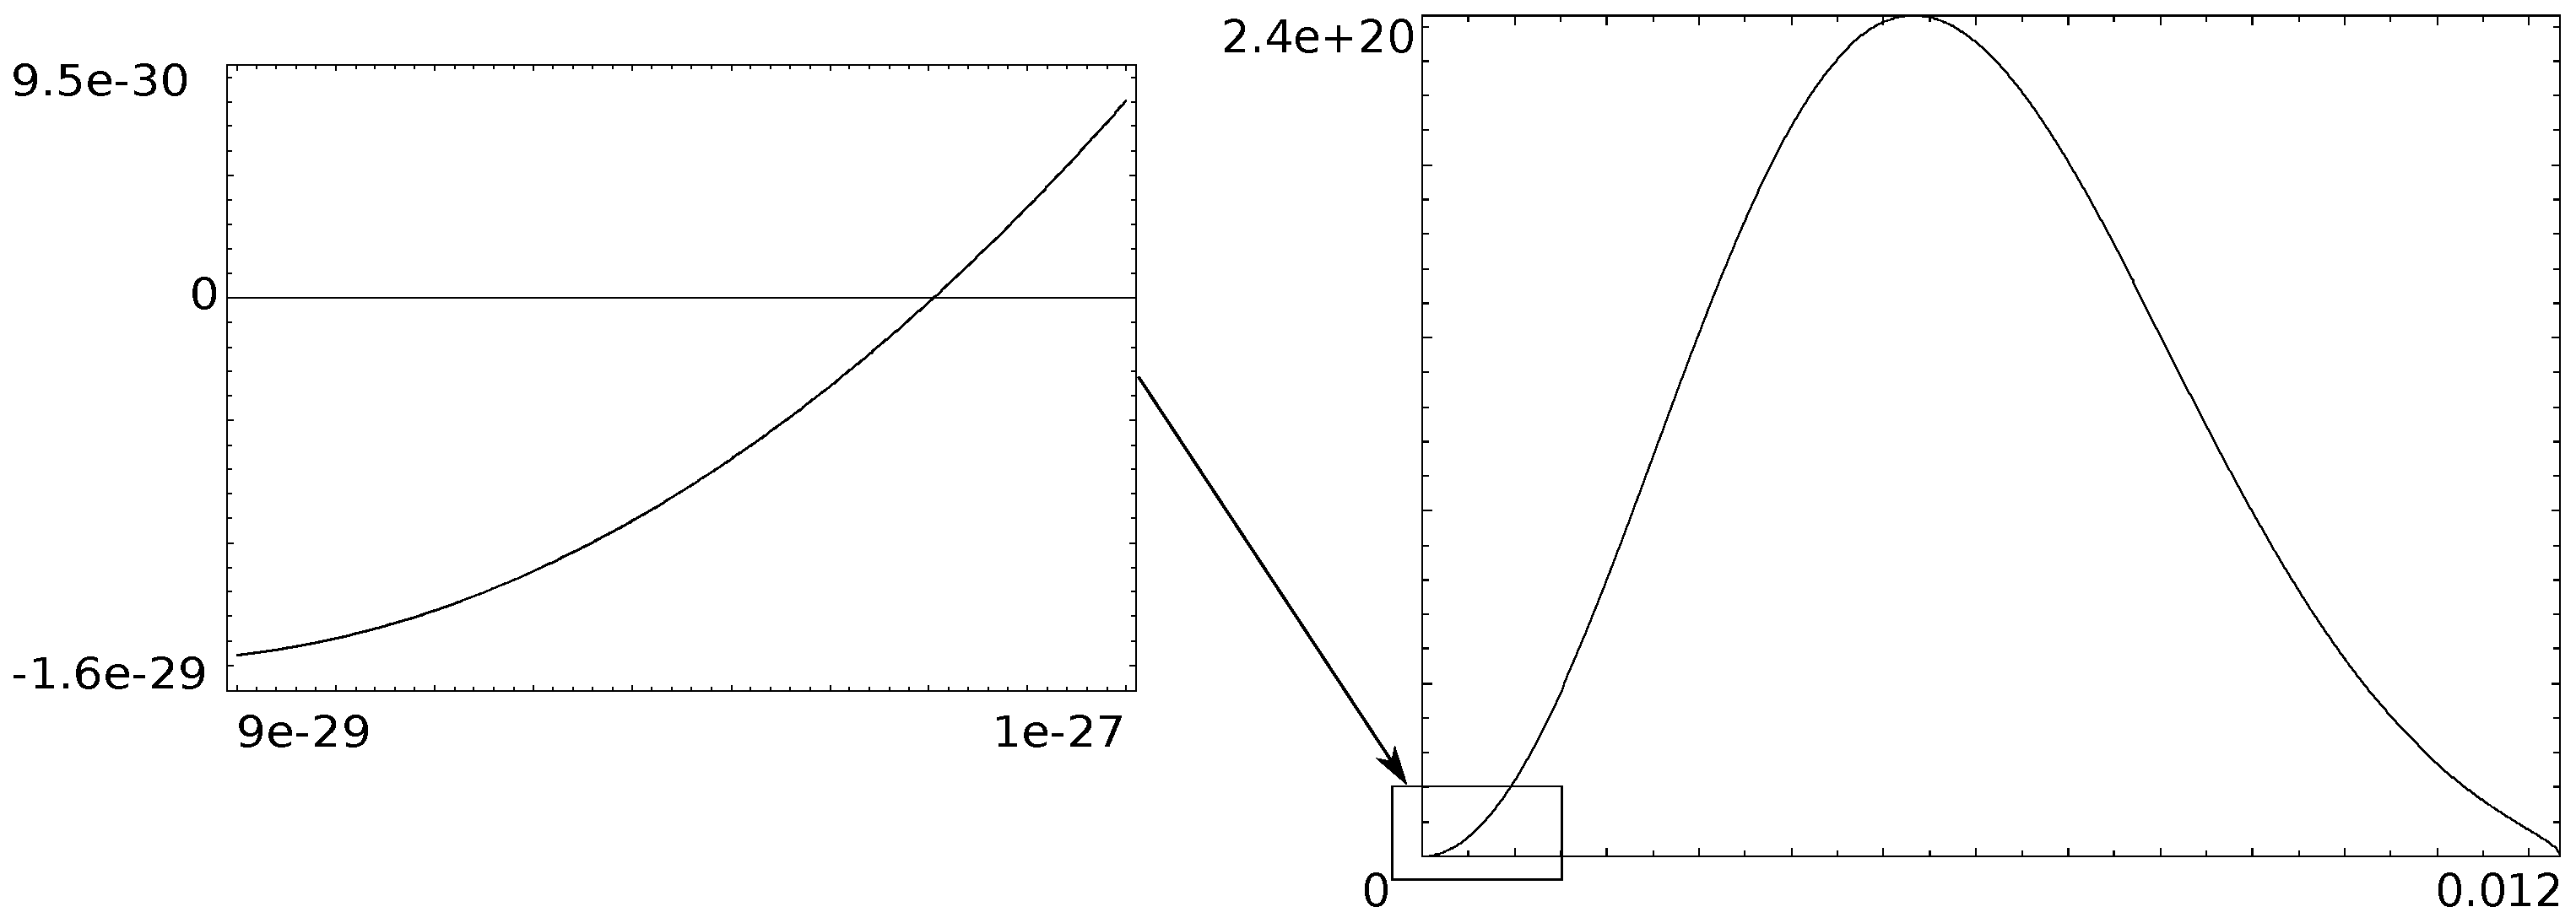
\includegraphics[width=11cm]{full.eps}
   \caption{Левая часть трансцендентного уравнения относительно $\lambda$}
  \end{figure}
\end{frame}

\begin{frame}
 \frametitle{Анимация процесса}
 Выберем значения переметров следующим образом:
  \begin{equation*}
    l_1=3,\ l_2=5,\ a_1=2,\ a_2=4,\ w_1=0.1,\ w_2=w_1 \cdot 0.8.
  \end{equation*}
 \begin{center}
   \animategraphics[controls, loop,height=5cm]{100}{a1/animation-one-}{1}{200} 
 \end{center}
\end{frame}


\begin{frame}
 \frametitle{Анимация процесса}
 Выберем значения переметров следующим образом:
  \begin{equation*}
    l_1=3,\ l_2=1,\ a_1=4,\ a_2=1,\ w_1=0.05,\ w_2=w_1 \cdot 0.8.
  \end{equation*}
 \begin{center}
   \animategraphics[controls, loop,height=5cm]{100}{a2/animation-two-}{1}{200} 
 \end{center}
\end{frame}

\begin{frame}
 \frametitle{Анимация процесса}
 Сравним процесс с конвекцией (слева) и без конвекции (справа):
 \begin{center}
   \animategraphics[controls, loop,height=4cm]{100}{a3/animation-four-}{1}{200} 
 \end{center}
\end{frame}

\end{document}
